\section{Results Analysis}

\begin{figure}[t]
\centering
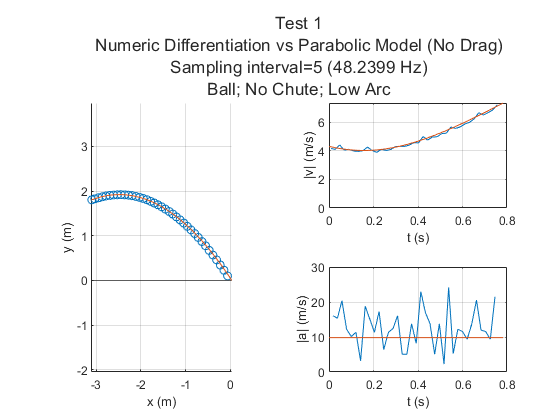
\includegraphics[width=0.9\linewidth]{images/Analysis1_Test1_Fig5_NoDrag.png}
\caption{\label{fig:Analysis1_Test1_Fig5_NoDrag} Fitting the parabolic model to sampled position data for a ball with no parachute. On the right you see the velocity and acceleration computed using numeric differentiation (blue) and the model's velocity and acceleration (orange). For low-drag scenarios, the parabolic model appears adequate.}
\end{figure}

So how does the parabolic model perform? We started by running it on some data of just the plain ball with no parachute attached, thrown in a low arc to minimize drag effects. The data is shown in Fig.~\ref{fig:Analysis1_Test1_Fig5_NoDrag}. 